\documentclass{beamer}
\graphicspath{{images/}}
%PDF-Dokumente einbinden
\usepackage{pdfpages}
\usepackage{tikz}
\usetikzlibrary{shapes,arrows,automata,matrix}
\usetikzlibrary{decorations.pathreplacing,calc,positioning}
\usetikzlibrary{dsp,chains}
\usepackage{tikz-timing}[2009/12/09]
\usetikztiminglibrary[new={char=Q,reset char=R}]{counters}
\usetikzlibrary{decorations,arrows} 
\usetikzlibrary{decorations.pathmorphing} 
\usepgflibrary{decorations.pathreplacing} 

\usepackage[utf8]{inputenc}
\usepackage[ngerman]{babel}
\usepackage{pgf}
\usepackage[OT1]{fontenc} % Ligaturen, richtige Umlaute im PDF
%Umschalten der Sprache
\selectlanguage{ngerman}
\newcommand{\fullname}{Andreas Rehn}
\newcommand{\titel}{Ultraschallgerät zur definierten Messung von Strömungsprofilen in einem Schlauch basierend auf einem Embedded System}
%was ist definiert
\usetheme{Dresden}
\beamertemplatenavigationsymbolsempty
%\setbeamercovered{transparent}
\usepackage{bbding}
\newcommand*\tick{\item[\Checkmark]}
\newcommand*\fail{\item[\XSolidBrush]}

\tikzset{%
  block/.style    = {draw, , rectangle, minimum height = 3em,
    minimum width = 3em},
  sum/.style      = {draw, circle, node distance = 2cm}, % Adder
  input/.style    = {coordinate}, % Input
  output/.style   = {coordinate}, % Output
  right iso/.style={isosceles triangle,scale=0.5,sharp corners, anchor=center, xshift=-4mm},
  left iso/.style ={right iso, rotate=180, xshift=-8mm},
  txt/.style	  ={text width=1.5cm,anchor=center},
  ellip/.style	  ={ellipse,scale=0.5},
  empty/.style	  ={draw=none}
}

\tikzstyle{block} = [draw, rectangle, 
    minimum height=3em, minimum width=6em]
\tikzstyle{sum} = [draw, fill=blue!20, circle, node distance=2cm]
\tikzstyle{input} = [coordinate]
\tikzstyle{output} = [coordinate]
\tikzstyle{pinstyle} = [pin edge={to-,thin,black}]

\usepackage{pgfplots}
\pgfplotsset{width=7cm,compat=1.8}

\begin{document}

\title{\titel}
\author[A. Rehn]{\fullname}
\institute[IMM - HS Ulm]{Fakultät Mechatronik und Medizintechnik\\ Hochschule Ulm}
\titlegraphic{
\includegraphics[width=0.14\textwidth]{logo}}
\date[17.03.15]{17. März 2015}

\frame{\titlepage}

\expandafter\def\expandafter\insertshorttitle\expandafter{%
  \insertshorttitle\hfill\insertframenumber}%\,/\,\inserttotalframenumber}
  
\logo{\pgfimage[width=0.14\textwidth]{images/logo}}
%\setbeamertemplate{footline}[frame number]
\frame{\frametitle{Agenda}
	\tableofcontents
	[pausesections]
}

\section{Thema}

\subsection{Motivation}
\begin{frame}
\logo{
\includegraphics[height=0.3]{logo}}
Hämatokritwert := Volumenanteil roter Blutkörperchen im Blut
\begin{block}{invasive Hämatokritbestimmung mit Zentrifugation}
	\begin{itemize}
		\item permanente Kosten
		\item erhöhte Auswertungszeit
	\end{itemize}
\end{block}
\begin{block}{nicht invasive Hämatokritbestimmung mit Sonographie}
	\begin{itemize}
		\item erhöhte Investitionskosten
		\item echtzeitnahe Auswertung und Visualisierung
	\end{itemize}
\end{block}

\end{frame}

\subsection{Aufgabenstellung}
\begin{frame}
\begin{columns}
	\column{.4\textwidth} 
		\begin{figure}[h]
			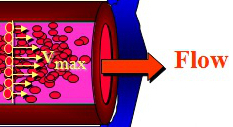
\includegraphics[width=1\textwidth]{pw/flowProfil}
		\end{figure}
	\column{.6\textwidth}
	\begin{itemize}
		\only<1>{
			\item Erfassung von Strömungsprofilen $\upsilon(r)=?$
			\item nicht invasiv
		}
		\only<2>{
			\item Erfassung von Strömungsprofilen $\upsilon(r)=?$
			\item nicht invasiv \Checkmark
		}
		\only<3>{
			\item Erfassung von Strömungsprofilen $\upsilon(r)=?$ \Checkmark
			\item nicht invasiv \Checkmark
		}
	\end{itemize}
	\end{columns}
\only<2>{\begin{columns}
	\column{.4\textwidth} 
		\begin{figure}[h]
			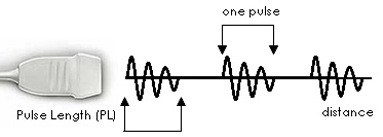
\includegraphics[width=1\textwidth]{pw/pulselength}
		\end{figure}
	\column{.6\textwidth}
		\begin{block}{Technologie pulsed wave Ultrasonic Doppler}
		\begin{itemize}			
			\item[\Checkmark] longitudinale Ausbreitung
			\item[\Checkmark] Frequenzen von 2 bis 8 MHz			
			\item[\Checkmark] variable Energie/ -dichte
			\item[\Checkmark] Gewebetiefen bis 80 mm
		\end{itemize}
		\end{block}
	\end{columns}}

\only<3>{\begin{columns}
	\column{.4\textwidth} 
		\begin{figure}[h]
			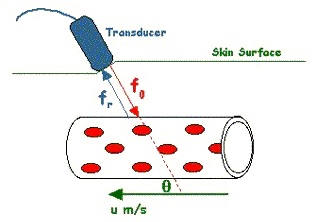
\includegraphics[width=1\textwidth]{pw/DopplerBloodFlow}
		\end{figure}
	\column{.6\textwidth}
		\begin{block}{Strömungsprofilermittlung basierend auf Doppereffekt}
		\begin{itemize}
			\item $\Delta f= f_0-f= \dfrac{2f_0\cdot cos\left(\theta\right)}{\upsilon}$
			\item[\Checkmark] $\upsilon=\dfrac{2f_0\cdot cos\left(\theta\right)}{\Delta f}$
		\end{itemize}
		\end{block}
	\end{columns}}
\end{frame}

\input{praesi_overview}

\section{Realisierung}
\subsection{Receiver Bandpass}
\begin{frame}
\begin{tikzpicture}[auto, node distance=3cm,>=latex, scale=0.56, transform shape]
    % We start by placing the blocks
%    \node [input, name=input] {};

    \node [input] (sum) {};
    \node [block, right of=sum, fill=blue!20] (filter) {Bandpass};
    \node [block, right of=filter,
    		node distance=4cm] (controller) {Verstärker};
    \node [block, right of=controller, %pin={[pinstyle]above:Disturbances},
            node distance=4cm] (system) {ADC};
    \node [block, right of=system,
    		node distance=4cm] (pld) {CPLD};
    \draw[decorate,decoration={brace, mirror}] ([yshift=-10pt]filter.south west) -- ([yshift=-10pt]system.south east) node at (7,-1.2) [below]{Receiver} ; 
    % We draw an edge between the controller and system block to 
    % calculate the coordinate u. We need it to place the measurement block. 
    \draw [->] (controller) -- node {?} (system);
    \node [output, right of=system] (output) {};
%    \node [block, below of=u] (measurements) {Measurements};

    % Once the nodes are placed, connecting them is easy. 
%    \draw [draw,->] (input) -- node {$r$} (sum);
    \draw [->] (sum) -- node {?} (filter);
    \draw [->] (filter) -- node {?} (controller);
    \draw [->] (system) -- node {?} (pld);
%    \draw [->] (y) |- (measurements);
%    \draw [->] (measurements) -| node[pos=0.99] {$-$} 
%        node [near end] {$y_m$} (sum)
;
\end{tikzpicture}
\end{frame}

\begin{frame}
\begin{block}{Rahmenbedingungen}
\begin{itemize}
	\item Trägerfrequenz von 2, 4, 8 MHz
	\item $\Delta f \approx \pm$ 50 Hz \ldots 10 kHz
	\item Dämpfung = const; $\Rightarrow$ Eindringtiefe $\searrow$ Trägerfrequenz $f_0$ $\nearrow$
	\item statische und dynamische Echos
\end{itemize}
\end{block}
\visible<2->{\begin{block}{Definition Parameter}
\begin{itemize}
	\item untere Grenzfrequenz $f_L=100$ kHz\only<2->{\footnote{max. Burst Länge von 10 $\mu$s}}
	\item obere Grenzfrequenz $f_H=8$ MHz
	\item minimale Dämpfung bei 2 MHz
	\item starke Dämpfung $\Rightarrow$ Bandpass 2. Ordnung
\end{itemize}
\end{block}}
\end{frame}

\begin{frame}
\begin{figure}
			\centering
		   	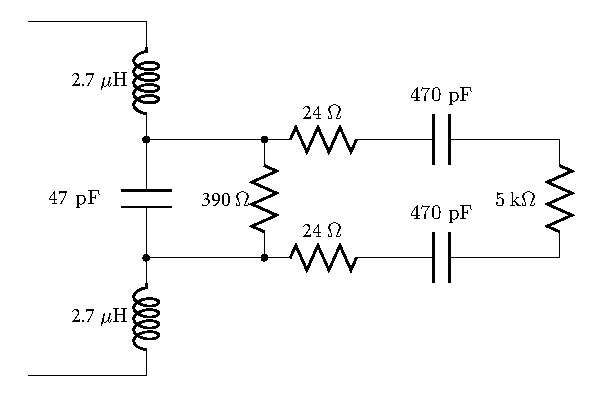
\includegraphics[width=\textwidth]{images/Bandpass/full}
	    		\caption{realisierbare Schaltung des Filters}
	    		\label{fig:filter_full}
	\end{figure}
\end{frame}
\begin{frame}
			\begin{figure}
			\includegraphics[width=0.9\textwidth]{images/Bandpass}
		    \caption{Verhalten des Filters}
		    \label{fig:filter_verhalten}
			\end{figure}
\end{frame}

\subsection{Receiver Verstärker}
\begin{frame}
\begin{tikzpicture}[auto, node distance=3cm,>=latex, scale=0.56, transform shape]
    % We start by placing the blocks
%    \node [input, name=input] {};

    \node [input] (sum) {};
    \node [block, right of=sum] (filter) {Bandpass \Checkmark};
    \node [block, right of=filter,
    		node distance=4cm, fill=blue!20] (controller) {Verstärker};
    \node [block, right of=controller, %pin={[pinstyle]above:Disturbances},
            node distance=4cm] (system) {ADC};
    \node [block, right of=system,
    		node distance=4cm] (pld) {CPLD};
    \draw[decorate,decoration={brace, mirror}] ([yshift=-10pt]filter.south west) -- ([yshift=-10pt]system.south east) node at (7,-1.2) [below]{Receiver} ; 
    % We draw an edge between the controller and system block to 
    % calculate the coordinate u. We need it to place the measurement block. 
    \draw [->] (controller) -- node {?} (system);
    \node [output, right of=system] (output) {};
%    \node [block, below of=u] (measurements) {Measurements};

    % Once the nodes are placed, connecting them is easy. 
%    \draw [draw,->] (input) -- node {$r$} (sum);
    \draw [->] (sum) -- node {?} (filter);
    \draw [->] (filter) -- (controller);
	\draw [->] (system) -- node {?} (pld);
%    \draw [->] (y) |- (measurements);
%    \draw [->] (measurements) -| node[pos=0.99] {$-$} 
%        node [near end] {$y_m$} (sum)
;
\end{tikzpicture}\end{frame}

\begin{frame}
\begin{block}{Rahmenbedingungen}
\begin{itemize}
\item max. ADC Eingangsbereich von 2 Vpp (differenziell)
\item Innenwiderstand der Sonde variiert von 20 bis 80 $\Omega$
\item max. Ausnutzung des ADC Eingangsbereichs\\ bei einem max. Sensorsignal mit 100 mVpp Amplitude
\item 5 \% Toleranz bei Widerständen der E12 Reihe
\end{itemize}
\end{block}
\begin{block}{Definition Parameter}
\begin{itemize}
	\item Innenwiderstand der Sonde wird auf 50 $\Omega$ definiert
	\item min. Verstärkung von 26 dB benötigt
\end{itemize}
\end{block}
\end{frame}

\begin{frame}
\begin{tikzpicture}[auto, node distance=3cm,>=latex, scale=0.56, transform shape]
    % We start by placing the blocks
%    \node [input, name=input] {};

    \node [input] (sum) {};
    \node [block, right of=sum] (filter) {Bandpass \Checkmark};
    \node [block, right of=filter,
    		node distance=4cm] (controller) {Verstärker};
    \node [block, right of=controller, %pin={[pinstyle]above:Disturbances},
            node distance=4cm] (system) {ADC};
    \node [block, right of=system,
    		node distance=4cm] (pld) {CPLD};
    \draw[decorate,decoration={brace, mirror}] ([yshift=-10pt]filter.south west) -- ([yshift=-10pt]system.south east) node at (7,-1.2) [below]{Receiver} ; 
    % We draw an edge between the controller and system block to 
    % calculate the coordinate u. We need it to place the measurement block. 
    \draw [->] (controller) -- node[name=u] {2 Vpp} (system);
    \node [output, right of=system] (output) {};
%    \node [block, below of=u] (measurements) {Measurements};

    % Once the nodes are placed, connecting them is easy. 
%    \draw [draw,->] (input) -- node {$r$} (sum);
    \draw [->] (sum) -- node {100 mVpp} (filter);
    \draw [->] (filter) -- (controller);
	\draw [->] (system) -- node {?} (pld);
%    \draw [->] (y) |- (measurements);
%    \draw [->] (measurements) -| node[pos=0.99] {$-$} 
%        node [near end] {$y_m$} (sum)
;
\end{tikzpicture}
\visible<2->{\begin{figure}
	\centering
	\includegraphics[width=.8\textwidth, trim=13mm 194mm 111mm 50mm, clip=true]{images/AD8351}
%	\caption{Low Distortion Differential RF/IF Amplifier AD8351}
\end{figure}}

\end{frame}

\begin{frame}
\begin{columns}
	\column{.6\textwidth} 
		\begin{figure}[h!]
	\centering
	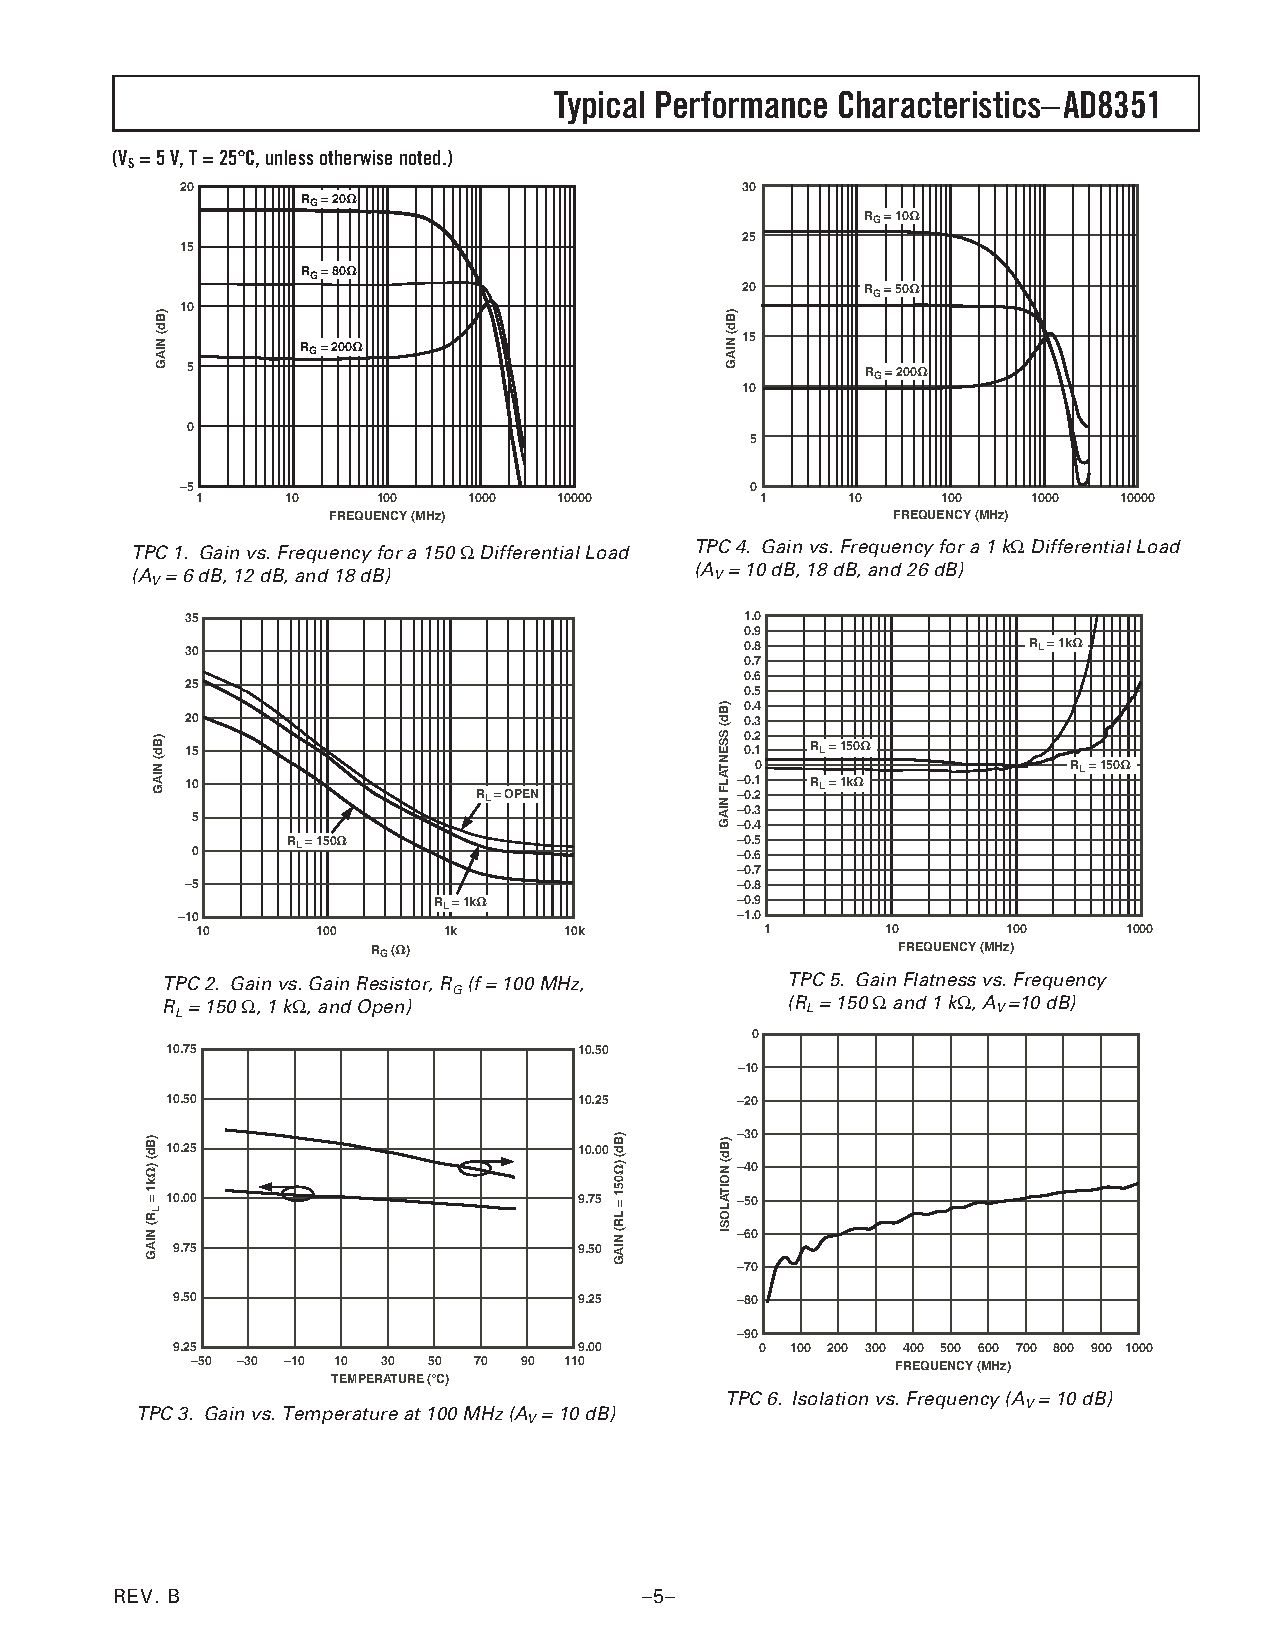
\includegraphics[width=1\textwidth, trim=115mm 180mm 15mm 30mm, clip=true]{images/Gain}
%	\caption{Verstärkung in Abhängigkeit vom Verstärkungswiderstand R$_G$}
	\label{fig:graph_gain}
\end{figure}
	\column{.4\textwidth}
	\begin{itemize}
		\visible<2->{\item theoretisch: 10 $\Omega$}
		\visible<3->{\item experimentell: 8 $\Omega$}
	\end{itemize}
\end{columns}

\end{frame}

\subsection{Signal-Rausch-Verhältnis}

\begin{frame}{ADC Parameter}
\begin{itemize}
	\item 14 bit Auflösung
	\item 65 Msps (8 Stützstellen für 8 MHz Trägerfrequenz)
	\item 2 Vpp Eingangsbereich
	\item $\approx$ 72 dB SNR
	%\item $\approx$ 88 dBc SFDR%\footnote{Spurious-free dynamic range}
\end{itemize}
\begin{tikzpicture}[auto, node distance=3cm,>=latex, scale=0.56, transform shape]
    % We start by placing the blocks
%    \node [input, name=input] {};

    \node [input] (sum) {};
    \node [block, right of=sum, fill=blue!20] (filter) {Bandpass \Checkmark};
    \node [block, right of=filter,
    		node distance=4cm, fill=blue!20] (controller) {Verstärker \Checkmark};
    \node [block, right of=controller, %pin={[pinstyle]above:Disturbances},
            node distance=4cm, fill=blue!20] (system) {ADC \Checkmark};
    \node [block, right of=system,
    		node distance=4cm] (pld) {CPLD};
    \draw[decorate,decoration={brace, mirror}] ([yshift=-10pt]filter.south west) -- ([yshift=-10pt]system.south east) node at (7,-1.2) [below]{Receiver} ; 
    % We draw an edge between the controller and system block to 
    % calculate the coordinate u. We need it to place the measurement block. 
    \draw [->] (controller) -- node[name=u] {2 Vpp} (system);
    \node [output, right of=system] (output) {};
%    \node [block, below of=u] (measurements) {Measurements};

    % Once the nodes are placed, connecting them is easy. 
%    \draw [draw,->] (input) -- node {$r$} (sum);
    \draw [->] (sum) -- node {100 mVpp} (filter);
    \draw [->] (filter) -- (controller);
    \draw [->] (system) -- node [name=y] {14 bit}(pld);
%    \draw [->] (y) |- (measurements);
%    \draw [->] (measurements) -| node[pos=0.99] {$-$} 
%        node [near end] {$y_m$} (sum)
;
\end{tikzpicture}
\end{frame}
\begin{frame}{Bestimmung SNR und SFDR (1)}
\begin{figure}[b]
	\centering
  	\includegraphics[trim = 85mm 202mm 1.3cm 27mm, clip=true, width=.85\textwidth]{vortrag/SFDR_SNR}  
  	\caption{Spektrogramm}
  \end{figure}
\end{frame}

\begin{frame}{Bestimmung SNR und SFDR(2)}
\begin{columns}
	\column{1\textwidth} 
	\begin{enumerate}
\item FFT mit 512 Werten
\item Bestimmung der Fundamentalen (Trägerfrequenz)
\item $Noise=\sum_{n=1}^{N=256} Magnitude(n\cdot \Delta f) - Fundamental$
\item $SNR=20\cdot log_{10}\left(Fundamental/\sqrt{Noise}\right)$
\item $SFDR=20\cdot log_{10}\left(Fundamental/highest\  Spurious\right)$
\end{enumerate}
	\column{.0\textwidth}
\end{columns}
	
\end{frame}

\begin{frame}{Ergebnisse}

\begin{tikzpicture}
\begin{axis}[
    ybar,
    title={200 mVpp Eingansamplitude, 64 Msps},
    enlargelimits=0.25,
    bar width=26pt,
    width=1\textwidth,
    height=0.75\textheight,
    legend style={at={(0.5,-0.15)},
      anchor=north,legend columns=4},
    ylabel={power in dB},
    symbolic x coords={2 MHz,4 MHz,8 MHz},
    xtick=data,
    cycle list={
    {fill=black!60,draw=black!60},
    {fill=black!40,draw=black!40},
    {fill=black!20,draw=black!20}
},
    nodes near coords,
    nodes near coords align={vertical},
    ]
\addplot coordinates {(2 MHz,55.46) (4 MHz,51.92) (8 MHz,46.20)};
\addplot coordinates {(2 MHz,58.74) (4 MHz,51.30) (8 MHz,49.93)};
\addplot coordinates {(2 MHz,60.83) (4 MHz,53.35) (8 MHz,50.54)};
\legend{Matlab SNR,Matlab SFDR,Matlab Skript}
\end{axis}
\end{tikzpicture}
\end{frame}


\subsection{Demodulierung und Bildgebung}
\begin{frame}[fragile]
\begin{figure}[h!t]
\centering
\begin{tikzpicture}
	\matrix (m0) [row sep=2.5mm, column sep=12mm]
	{	%--------------------------------------------------------------------
		\node[coordinate]                  (m00) {};   		  &
		\node[coordinate]                  (m01) {};   		  &
		\node[dspmixer]                    (m02) {};   		  &
		\node[dspsquare]                   (m03) {LPF};   	  &
		\node[dspnodeopen,dsp/label=below] (m0X) {$I[n]$};	  \\				%--------------------------------------------------------------------
		\node[dspnodeopen,dsp/label=above] (m10) {$r[n]$};    &
		\node[dspnodefull]                 (m11) {};          &
		\node[coordinate]                  (m12) {};          &
		\node[coordinate]                  (m13) {};          &
		\node[coordinate]                  (m1X) {};          \\		%--------------------------------------------------------------------
		\\		%--------------------------------------------------------------------
		\node[coordinate]                  (m20) {};          &
		\node[coordinate]                  (m21) {};          &
		\node[dspmixer]                    (m22) {};   		  &
		\node[dspsquare]                   (m23) {LPF};		  &
		\node[dspnodeopen,dsp/label=below] (m2X) {$Q[n]$};    \\		%--------------------------------------------------------------------		%--------------------------------------------------------------------
		\node[coordinate] (m30) {}; &
		\node[coordinate] (m31) {}; &
		\node[coordinate] (m32) {}; &
		\node[coordinate] (m33) {}; &
		\node[coordinate] (m3X) {};    \\		%--------------------------------------------------------------------
	};	
	\begin{scope}[start chain]
		\chainin (m10);
		\chainin (m11) [join=by dspconn];
		\chainin (m01) [join=by dspline];
		\chainin (m21) [join=by dspline];
	\end{scope}
	\draw[dspconn]  (m12) -- node[below] {$cos(2\pi f_0n)$} (m02);	
	\draw[dspconn]  (m32) -- node[below] {$sin(2\pi f_0n)$} (m22);	
			
	\foreach \i [evaluate = \i as \j using int(\i+1)] in {1,..., 2}
	{
		\draw[dspconn] (m0\i) -- (m0\j);
		\draw[dspconn] (m2\i) -- (m2\j);
	}
	\draw[dspflow] (m03) -- (m0X);
	\draw[dspflow] (m23) -- (m2X);
\end{tikzpicture}
\caption{Blockdiagramm Quadraturdemodulation bestehend aus Down-Mixing und Tiefpass}
\end{figure}
\end{frame}

\begin{frame}
\begin{figure}[b]
	\centering
  	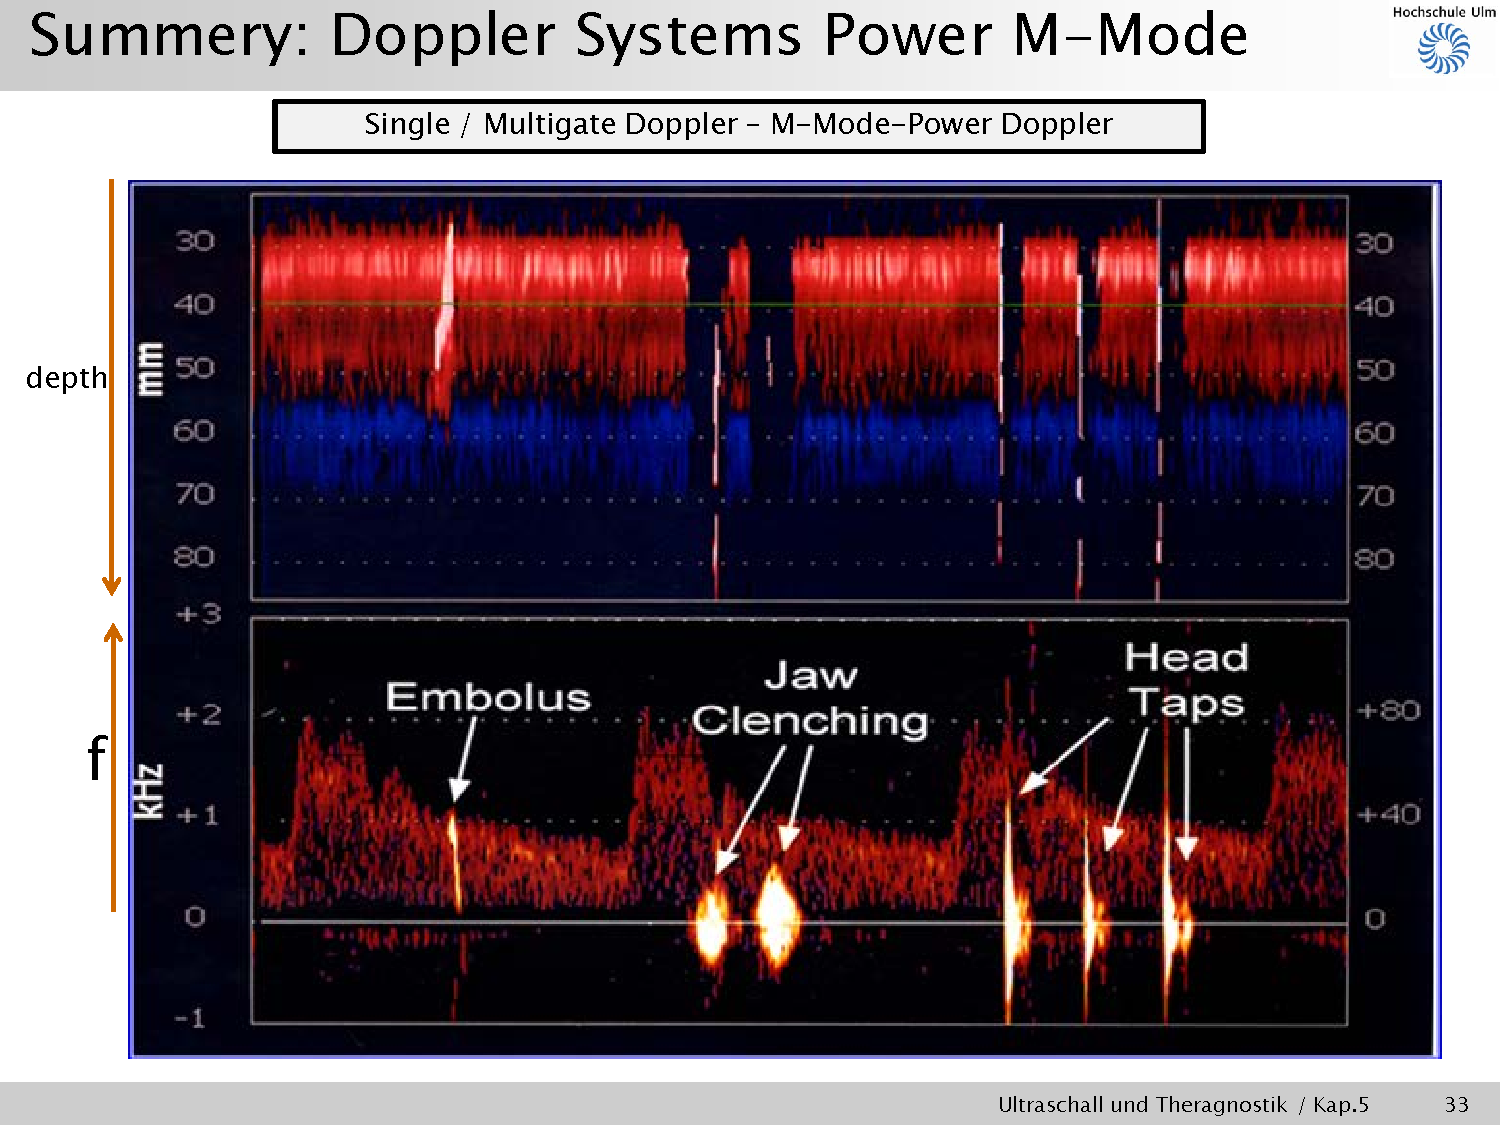
\includegraphics[trim = 2.2cm 1cm 1.3cm 3.5cm, clip=true, width=0.8\textwidth]{M-Mode}  
  	\caption{M-Mode mit Doppler Spektrogram}
  \end{figure}
\end{frame}

\begin{frame}
\begin{figure}[b]
	\centering
  	\includegraphics[trim = 1.3cm 19mm 1.6cm 28mm, clip=true, width=0.7\textwidth]{vortrag/Bildgebung}  
  	\caption{Quadraturdemodulation und Color Doppler processing}
  \end{figure}
\end{frame}

\section{Zusammenfassung}
\subsection{Ergebnisse}
\begin{frame}
\begin{itemize}
	\tick Analoge Signalaufbereitung (passiver Filter, Vorverstärker)
	\fail SNR zu gering
	\fail zu wenige Makro Zellen in CPLD um komplette Logik abzubilden
	\fail Datentransferrate wird von USB Full-Speed begrenzt
	\fail M-Mode Darstellung nicht optimal durch begrenzte Datentransferrate
	\tick Hämatokritwertbestimmung möglich
%	\item Projektziel ist mit Redesign und Komponentenaustausch realisierbar
%	\fail Projektziel konnte nicht realisiert werden
\end{itemize}
\end{frame}

\subsection{Ausblick}
\begin{frame}
\begin{itemize}
	\item Verbesserung des SNR durch PCB Redesign
	\item Offset Kompensation durch HPF nach CPLD Upgrade möglich
	\item Optimierung des M-Mode nach Erhöhung der Datentransferrate zwischen System und PC
	\item Zertifizierung und Nutzung für Gehirnoperationen
%	\item Emboliededektion
\end{itemize}
\end{frame}

\subsection*{Fragen}
\begin{frame}
Danke für Ihre Aufmerksamkeit!\\
\textbf{Fragen?}
\end{frame}

\end{document}
